% !TEX encoding = UTF-8 Unicode
\documentclass[a4paper]{article}

\usepackage{color}
\usepackage{url}
\usepackage[T2A]{fontenc} % enable Cyrillic fonts
\usepackage[utf8]{inputenc} % make weird characters work
\usepackage{graphicx}

\usepackage[english,serbian]{babel}
%\usepackage[english,serbianc]{babel} %ukljuciti babel sa ovim opcijama, umesto gornjim, ukoliko se koristi cirilica

\usepackage[unicode]{hyperref}
\hypersetup{colorlinks,citecolor=green,filecolor=green,linkcolor=blue,urlcolor=blue}

\usepackage{listings}

%\newtheorem{primer}{Пример}[section] %ćirilični primer
\newtheorem{primer}{Primer}[section]

\definecolor{mygreen}{rgb}{0,0.6,0}
\definecolor{mygray}{rgb}{0.5,0.5,0.5}
\definecolor{mymauve}{rgb}{0.58,0,0.82}

\lstset{ 
  backgroundcolor=\color{white},   % choose the background color; you must add \usepackage{color} or \usepackage{xcolor}; should come as last argument
  basicstyle=\scriptsize\ttfamily,        % the size of the fonts that are used for the code
  breakatwhitespace=false,         % sets if automatic breaks should only happen at whitespace
  breaklines=true,                 % sets automatic line breaking
  captionpos=b,                    % sets the caption-position to bottom
  commentstyle=\color{mygreen},    % comment style
  deletekeywords={...},            % if you want to delete keywords from the given language
  escapeinside={\%*}{*)},          % if you want to add LaTeX within your code
  extendedchars=true,              % lets you use non-ASCII characters; for 8-bits encodings only, does not work with UTF-8
  firstnumber=1000,                % start line enumeration with line 1000
  frame=single,	                   % adds a frame around the code
  keepspaces=true,                 % keeps spaces in text, useful for keeping indentation of code (possibly needs columns=flexible)
  keywordstyle=\color{blue},       % keyword style
  language=Python,                 % the language of the code
  morekeywords={*,...},            % if you want to add more keywords to the set
  numbers=left,                    % where to put the line-numbers; possible values are (none, left, right)
  numbersep=5pt,                   % how far the line-numbers are from the code
  numberstyle=\tiny\color{mygray}, % the style that is used for the line-numbers
  rulecolor=\color{black},         % if not set, the frame-color may be changed on line-breaks within not-black text (e.g. comments (green here))
  showspaces=false,                % show spaces everywhere adding particular underscores; it overrides 'showstringspaces'
  showstringspaces=false,          % underline spaces within strings only
  showtabs=false,                  % show tabs within strings adding particular underscores
  stepnumber=2,                    % the step between two line-numbers. If it's 1, each line will be numbered
  stringstyle=\color{mymauve},     % string literal style
  tabsize=2,	                   % sets default tabsize to 2 spaces
  title=\lstname                   % show the filename of files included with \lstinputlisting; also try caption instead of title
}

\begin{document}

\title{Razvoj Programskih Jezika u 2018.\\ \small{Seminarski rad u okviru kursa\\Metodologija stručnog i naučnog rada\\ Matematički fakultet}}

\author{ \href{mailto:dusan95kv@gmail.com}{Dušan Milović}, \href{mailto:dusanpilipovic95@gmail.com}{Dušan Pilipović}, \href{mailto:petricicmarko1995@gmail.com}{Marko Petričić}, \href{mailto:vido995@gmail.com}{Vido Mladenović}}

\date{April 2019.}

\maketitle

\abstract{
U ovom radu osvrnuli smo se na razvoj i nastanak novih okvira, tehnologija, koncepta i programskih jezika u poslednjih nekoliko godina, a posebno smo prokomentarisali njihovo stanje u 2018. godini. Obradili smo trenutno stanje u industriji, prokomentarisali tehnologije koje koriste najveće kompanije i izdvojili ono za šta se očekuje da bude u žiži interesovanja i u narednom periodu.}

\tableofcontents

\newpage

\section{Uvod}
\label{sec:uvod}

U današnje vreme život se ne može zamisliti bez modernih tehnologija. Potražnja za softverom je sve veća a broj ljudi koji imaju znanja da ga naprave nije tako veliki. Upravo ti ljudi koji razvijaju softvere se bave poslom koji je u poslednjih par godina jedan od najdinamičnijih poslova na svetu. Dinamika se ne ogleda u tome koliko treba fizički biti aktivan, već koliko je potrebno uložiti truda kako bi se ispratio razvoj svih tehnologija uz čiju pomoć razvijaju softvere. Upravo o tom razvoju ćemo pričati, o naglom skoku broja zainteresovanih za razvoj softvera kao i brzina razvoja tehnologija.

\section{Uloga industrije}
\label{sec:uloga industrije}

Bilo da se dvoumimo koji programski jezik da počnemo da učimo, ili u kojoj tehnologiji da započnemo novi projekat, veoma je važno da to što uradimo bude korisno i upotrebljivo i u narednom periodu. Programski jezik može da nastane, da se razvija i doživi ogromnu slavu i nakon toga da samo nestane i ne bude toliko popularan u svega godinu dana. Odabir tehnologije zavisi od prirode problema koji rešavamo ali i od ličnih zahteva i simpatija. Na mnogo načina možemo da poredimo programske jezike, ali doprinos boljoj odluci koju tehnologiju izabrati u velikoj meri može da predstavlja izučavanje šta je u centru pažnje u tehnološkoj industriji. Industrija će nam dati bitne trendove i znake koji će nam pomoći da donesemo odluku. Na primer ukoliko imamo informaciju da će određena tehnologija doneti najviše novca u 2018. godini ili da je najpopularnija u industriji, sigurno će nam skrenuti pažnju i povećati šanse da se usredsredimo baš na tu tehnologiju. U industriji je značajno više aspekata, pa ćemo se mi osvrnuti na tri najrelevantnija aspekta. Prvi o kojem ćemo pričati predstavlja količinu projekata u industriji koji su zasnovani na određenoj tehnologiji, zatim ćemo pomenuti tehnologije koje donose najlakšu zaposlenost i poslednje ali ne najmanje bitno koliko se isplati u finansijskom smislu koja tehnologija.

\subsection{Projekti}
\label{subsec:projekti}
Količina projekata u određenoj tehnologiji nam mnogo govori o toj tehnologiji i njenom razvoju. Iz toga možemo zaključiti pouzdanost tehnologije, njenu stabilnost, možemo shvatiti i koliko je isplativa ili neisplativa u zavisnosti od količine projekata. Loša strana posmatranja samo ovog pristupa može da bude to da u nekoj tehnologiji postoji veliki broj projekata, ali da je i veliki broj ljudi zna i koristi, pa možda potraga za poslom ne bude toliko jednostavan zadatak. I dalje ostaje otvoreno pitanje isplativosti te tehnologije jer možda ne zadovoljava lične zahteve i očekivanu dobit.

\subsubsection{Uticaj velikih kompanija}
\label{subsec:uticaj velikih kompanija}

Kao i u modi, tako i u svetu programiranja postoje nezvanični trend-seteri  u vidu velikih kompanija, čiji rad se neprestano prati i pokušavaju se izvući vrline koje čine te kompanije velikim. To su pre svega Microsoft, Facebook i Google, pa ćemo se osvrnuti na njihov rad i tehnologije koje najviše koriste. To nam predstavlja lep pokazatelj za tehnologiju da će verovatno biti veoma zastupljena u industriji.

\textbf{Microsoft.} Najpopularnija tehnologija koju razvijaju i koja je dosta primenjena je .NET. Ona podržava više objektno orijentisanih programskih jezika, C\#, F\#, Visual Basic \cite{dotnet}. Za web aplikacije pored .Net-a koriste dosta i Node.Js. Za razvoj hibridnih aplikacija React Native i Cordova alati \cite{webPlatforms}.

\textbf{Facebook.} Naravno prva asocijacija kada se pomene Facebook među programerima jeste React. Usled poteškoća oko održavanja svog koda za Facebook sajt, rodila se ideja o nastajanju framework-a za JavaScript koji je danas najpopularniji framework za web programiranje.

\textbf{Google.} Kao jedna od vodećih IT kompanija Google ima veliki uticaj na razvoj jezika. Između ostalog, oni su oformili i svoj jezik pa ćemo njega navesti kao prvog na spisku korišćenog u Google-u, reč je o GO jeziku. Na front-end strani najviše koriste JavaScript, dok na back-end delu pored GO-a koriste još C, C++, Java, Python \cite{google}.

\subsubsection{Uticaj novih interesovanja}
\label{subsec:Uticaj novih interesovanja}
Veliki izazov u industriji predstavlja analiza velike količine podataka. Sve je više informacija i podataka i potrebno ih je analizirati, sortirati i izvući ono najbitnije iz njih. Za čoveka bi to bilo veoma teško da uradi, pa se teži tome da računar odradi ceo posao. Odatle se razvijaju teme kao što su ''Big data'', Mašinsko učenje, Veštačka inteligencija... Razvoj tih tema uslovljava i razvoj određenih programskih jezika. U svetu mašinskog učenja i obrade velike količine podataka najzastupljeniji su Python i R.

\textbf{Python} je doživeo ogromnu porast u popularnosti tokom 2018. godine \cite{python}. Predočićemo Vam neke prednosti Python-a.
\begin{itemize}
    \item Python poseduje biblioteke koje su usmerene ka obradi podataka. To je jedini najveći razlog zašto se programeri sve više opredeljuju za Python. Nauka o podacima pruža zanimljiv posao koji je i veoma plaćen. Upoznaćemo se u kratkim crtama sa osnovnim bibliotekama Pythona namenjenih za oblast nauke o podacima:
    
    \textbf{Pandas:} Programska biblioteka pisana za Python u svrhu analize i manipulacije podacima. Pruža pogodne strukture podataka i operacije za manipulisanje numeričkim tabelama i vremenskim serijama. Reč je o besplatnom programskom izdanju izadatom pod okriljem 3-klauzulne BSD licence \cite{pandas}.
    
    \textbf{NumPy:} Ova biblioteka ima podršku za velike i višedimenzione nizove i matrice uporedo sa velikom kolekcijom matematičkih funkcija za operisanje nad ovim nizovima. Pandas je zasnovana na NumPy, i planirano je da se dobro uklapa sa ostalim naučnim kompjuterskim okruženjima tj nekim "3rd party" bibliotekama \cite{numPy}.
    
    \textbf{Matplotlib:} To je Python 2D biblioteka za grafikone koja proizvodi podatke o kvalitetu u različitim formatima. Može da se koristi u Python skriptama, u Python i IPython ''shell'', u Jupyter Notebook, u web aplikacijama \cite{matplotlib}.

    \item Mašinsko učenje je oblast koja sve više uzima maha u IT industriji. Algoritmi u ovoj oblasti postaju sve prefinjeniji. Google-ova pretraga je najpribližniji primer kako unapred pogađa šta želimo da pretražujemo. Ovo je razlog da svako koga zanima mašinsko učenje i veštačka inteligencija treba da nauče Python koji je u ovoj oblasti trenutno najdominantniji jezik.
\end{itemize}
    
    Gore navedene oblasti predstavljaju samo glavne prednosti učenja i rada u Python-u ali ne i jedine. Velika prednost Python-a jeste baš u tome što se ne koristi usko samo za jednu oblast, kao recimo R koji je dobar samo u analizi podataka i mašinskom učenju ali u web programiranju nema svoju primenu, dok Python i u web-u ima bilbioteke kao što su Django i Flask \cite{django, flask}.
    
    Prema anketama sa Stackoverflow-a na slici \ref{fig:PyhtonIndustry} je prikazano u kojim industrijama se najviše koristi Python.
    
\begin{figure}[h!]
\begin{center}
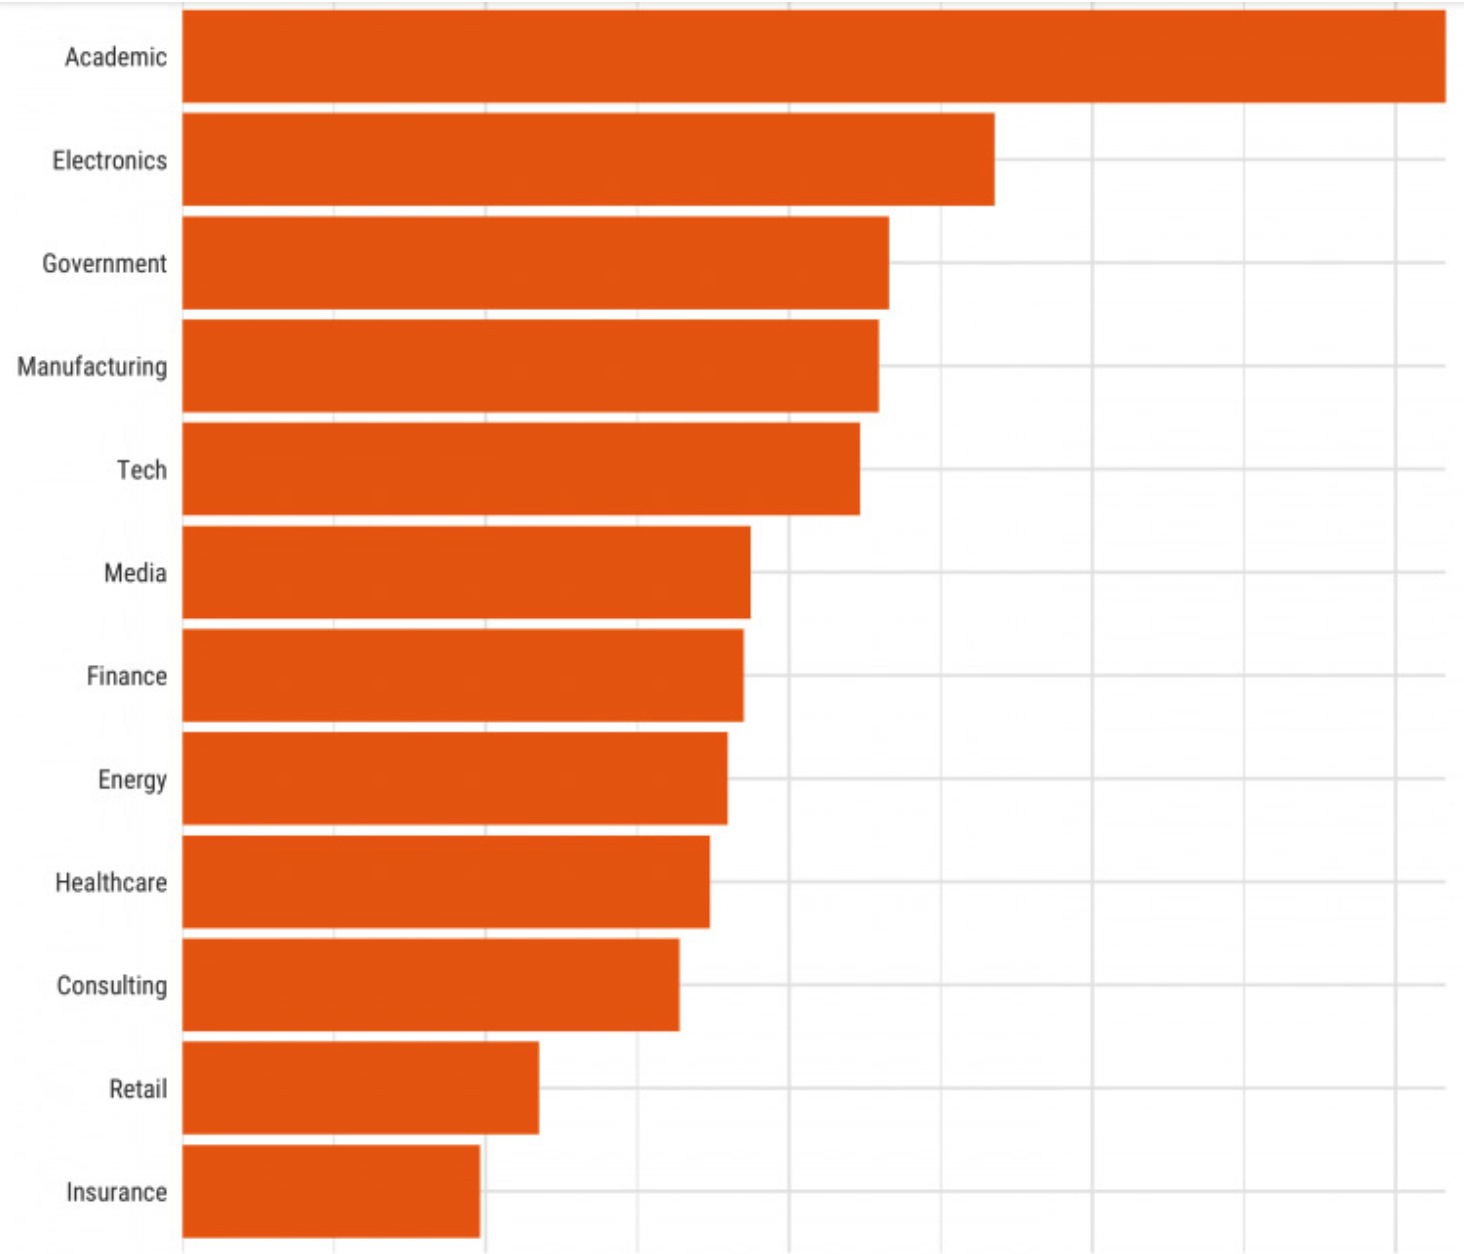
\includegraphics[scale=0.35]{slike/pythonIndustry.png}
\end{center}
\caption{Evidencija sa Stack Overflow-a o upotrebi Pythona u industriji}
\label{fig:PyhtonIndustry}
\end{figure}

Python je trenutno najbrže rastući jezik u oblasti analize podataka, a analiza podataka je trenutno najbrže rastuća oblast programiranja.

\subsection{Zaposlenost}
\label{subsec:zaposlenost}
Popularnost programskih jezika se može na različite načine porediti.
Smatramo da je najrelevantnija stopa zaposlenosti ljudi koji koriste određeni programski jezik. Da bismo prikazali stopu potražnje određenih programskih jezika u industriji, iskoristićemo analizu sprovedenu sa sajta Indeed.com (sajt za zapošljavanje) zasnovan na 25 programskih jezika, stack-ova, radnih okruženja \cite{indeed}.
Analiza je zasnovana na broju ponuda za posao za svaki programski jezik. Primetićete da neki jezici se ne nalaze na listi top 7 iako su među programerima popularni, kao što su Ruby i Swift. Slika \ref{fig:jobsIndeed}

\begin{figure}[h!]
\begin{center}
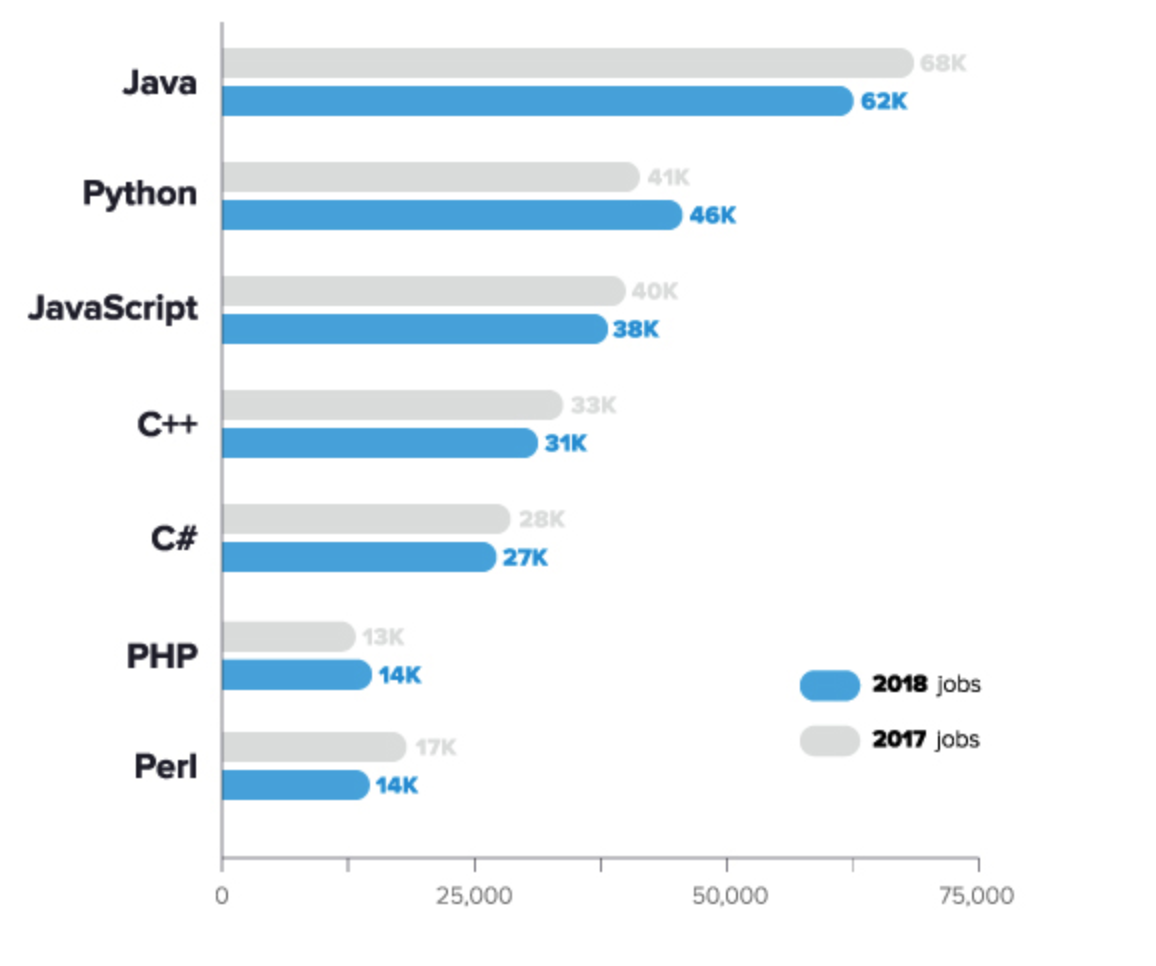
\includegraphics[scale=0.4]{slike/jobsIndeed.png}
\end{center}
\caption{Nivo zaposlenosti po tehnologijama}
\label{fig:jobsIndeed}
\end{figure}

\subsection{Isplativost}
\label{subsec:isplativost}
Za poslednju sekciju smo ostavili uticaj novca. Nije najmanje važna oblast, ali daleko i od toga da je najbitnija. Novac igra veliku ulogu u našim životima, medjutim naše finansijsko stanje ne zavisi od izbora tehnologije koju ćemo koristiti. Ako smo nečemu posvećeni, možemo dostići velike uspehe u skoro svakoj tehnologiji. Po analizama sa raznih sajtova imamo okvirno koje tehnologije u proseku donose koliko novca. Naravno treba uzeti u obzir da se standard u različitim državama može drastično razlikovati, pa bukvalno poređenje zarada nije adekvatno.

Prema sajtu Indeed.com \cite{salary} koji smo već spominjali kao jedan od vodećih sajtova za zapošljavanje situacija u USA na godišnjem nivou je kao na slici \ref{fig:salary1}.

\begin{figure}[h!]
\begin{center}
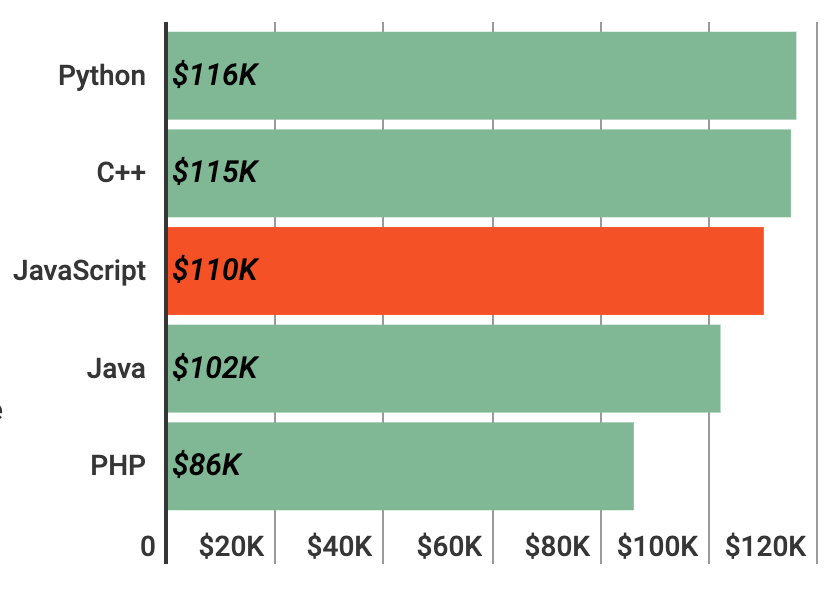
\includegraphics[scale=0.6]{slike/salary1.png}
\end{center}
\caption{Prosečna zarada u USA u odnosu na tehnologiju}
\label{fig:salary1}
\end{figure}

Na osnovu podataka sa Stackoverflow-a možemo uočiti da se situacija drastično menja ukoliko posmatramo količinu zarade širom sveta na godišnjem nivou, ne samo u USA. Slika \ref{fig:salary3}. 

\begin{figure}[h!]
\begin{center}
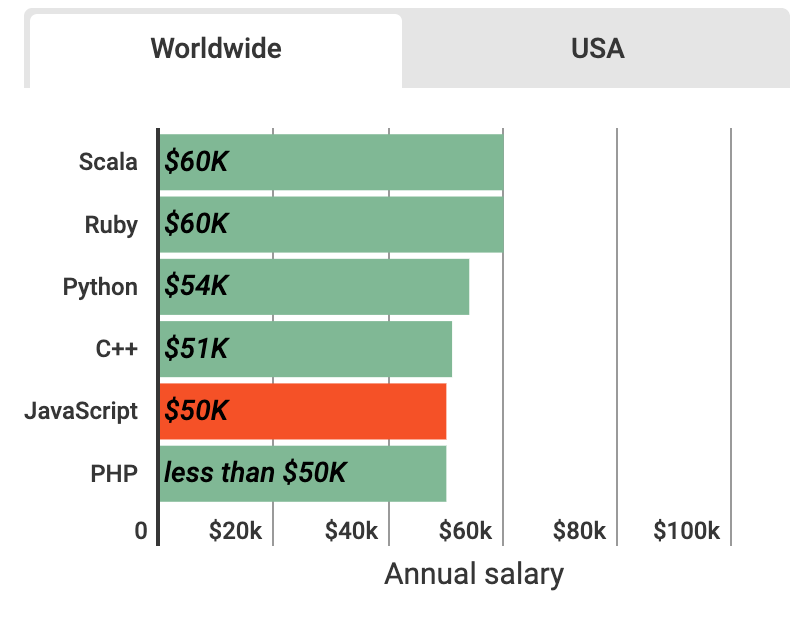
\includegraphics[scale=0.6]{slike/salary3.png}
\end{center}
\caption{Prosečna zarada u odnosu na tehnologiju širom sveta}
\label{fig:salary3}
\end{figure}

\section{Popularnost postojećih i nastanak novih jezika}
\label{sec:globalni razvoj}

Industrija programiranja se razvija pa tako i programski jezici. Istraživanja rađena na sajtu Github nam pokazuju u kojim programskim jezicima je rađeno najviše projekata, koji jezici su doživeli uspon, a koji pad u 2018. godini \cite{github}. Istraživanje je rađeno na osnovu mesečno aktivnih korisnika u proteklim godinama.

\subsection{Najpopularniji jezici}
\label{subsec:najpopularniji jezici}

\begin{figure}[h!]
\begin{center}
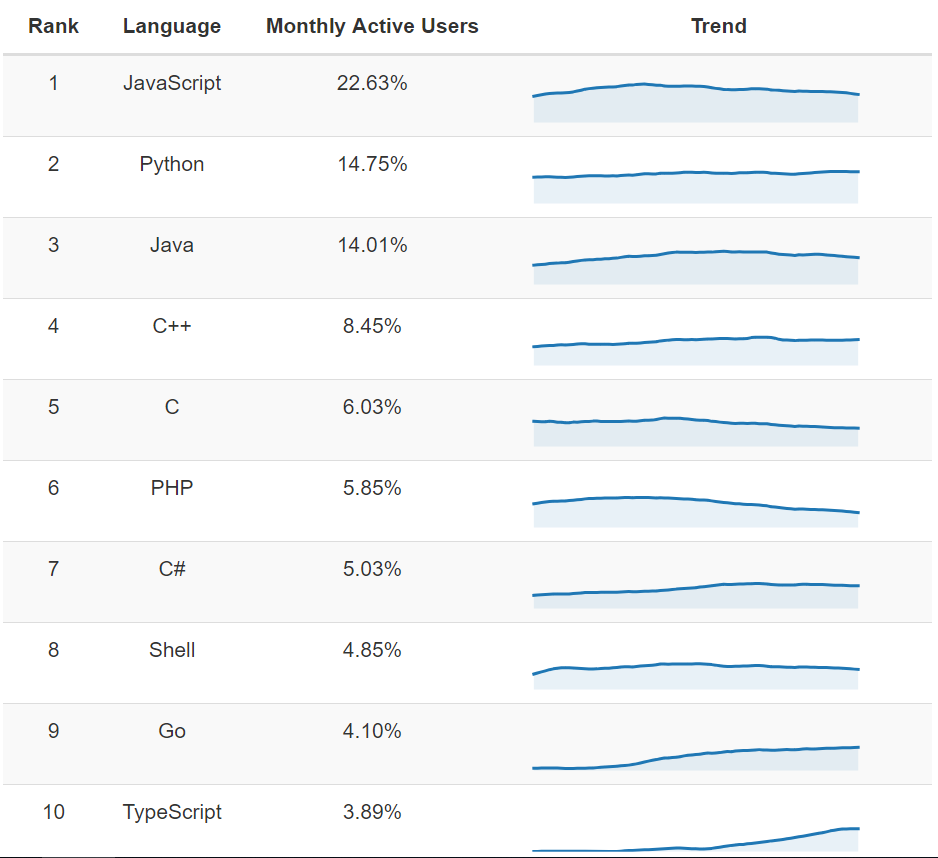
\includegraphics[scale=0.4]{slike/listaNajpopularnijihJezika.png}
\end{center}
\caption{Lista najpopularnijih jezika}
\label{fig:listaNajpopularnijihJezika}
\end{figure}

Lista najpopularnijih programskih jezika (slika \ref{fig:listaNajpopularnijihJezika}) nije se drastično promenila. Ovi jezici imaju relativno stabilnu upotrebu u proteklih par godina. JavaScript, Python, Java, C++ i C su najpopularniji jezici više od 8 godina i ne vidi se neka promena u skorije vreme.

JavaScript ostaje na prvom mestu najpopularnijih jezika uz pomoć brojnih framework-a koji su privukli još više korisnika.
Python vremenom raste i nedavno je prestigao Javu i postao drugi najpopularniji programski jezik. Kao što smo već spomenuli uspehu Python-a doprineo je nagli porast interesovanja u oblasti mašinskog učenja i ''Big data''.

\subsection{Noviji jezici}
\label{subsec:noviji jezici}

Jezici sa najbržim rastom broja korisnika u 2018. godini su Go, TypeScript, Kotlin i Rust. Slika \ref{fig:novijiJezici}

\begin{figure}[h!]
\begin{center}
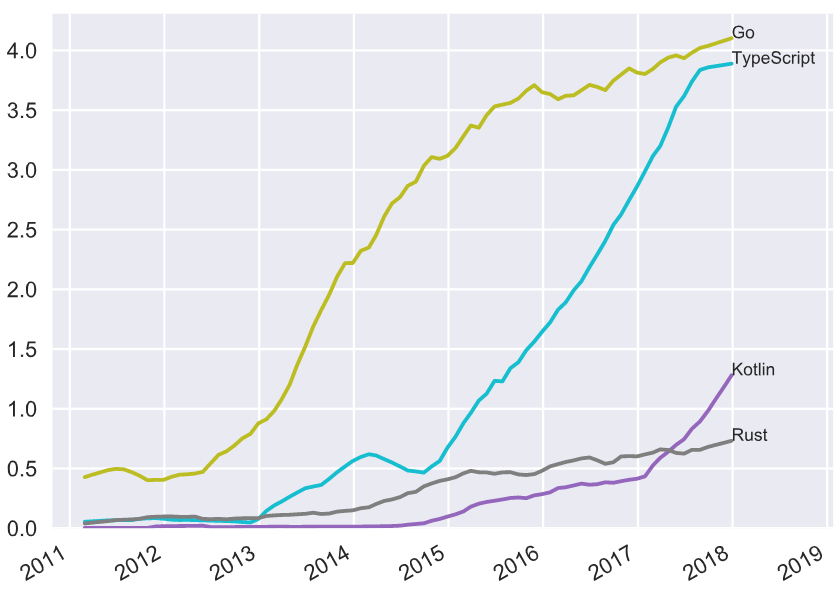
\includegraphics[scale=0.4]{slike/novijiJezici.png}
\end{center}
\caption{Noviji jezici}
\label{fig:novijiJezici}
\end{figure}

Kotlin se uglavnom koristi za razvoj Android aplikacija. Na grafu se može videti nagli porast korisnika kada je Google najavio punu podršku Kotlin-a na Android-u početkom 2017. godine.

Jedna zanimljiva stvar koja je zajednička za ove programske jezike je da ih sve sponzorišu velike kompanije: Google je pokrenuo Go, Microsoft TypeScript, JetBrains Kotlin i Mozilla Rust.

Stvaranje novog programskog jezika nije samo napraviti elegantan programski jezik za upotrebu. Treba razviti zajednicu i ekosistem iza jezika. Stvari kao što su podrška razvojnog okruženja, bibiloteke i paketi za uobičajne zadatke, alati i dokumentacije pomažu u stvaranju jezika i privlačenju velikog broja korisnika.

\subsection{Jezici koji su doživeli pad}
\label{subsec:pad jezika}

\begin{figure}[h!]
\begin{center}
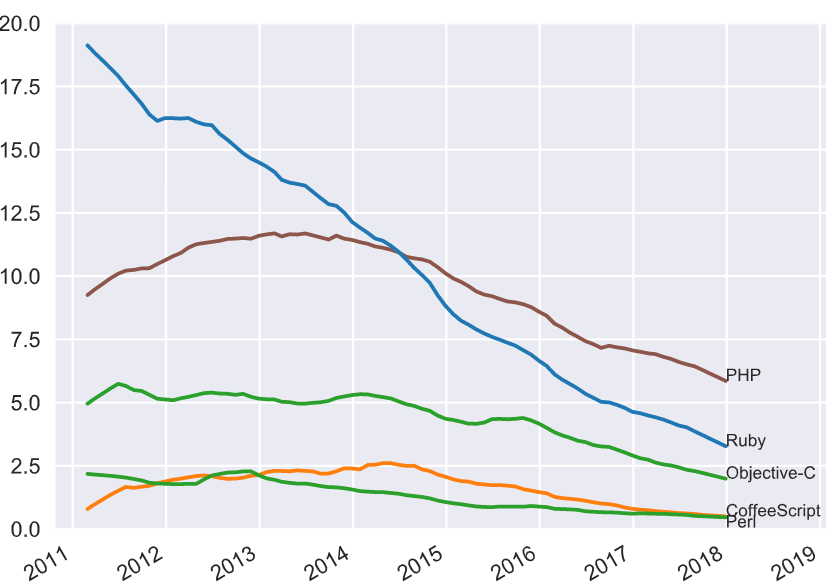
\includegraphics[scale=0.4]{slike/padJezika.png}
\end{center}
\caption{Jezici koji su doživeli pad u 2018.}
\label{fig:padJezika}
\end{figure}

Jezici kojima je opao broj korisnika u 2018. godini su Ruby, PHP, Objective-C, CoffeeScript i Perl (slika \ref{fig:padJezika}).
Ruby je zabeležio najveći pad u 2018. godini. Od 2. najpopularnijeg jezika u 2011. godini sa preko 18\% korisnika do 11. najpopularnijeg u 2018. sa svega 3,2\% korisnika. 

Pad korišćenja Objectiv-C odgovara porastu korišćenja Swift-a, dok je CoffeeScript zamenjen TypeScript-om. Dok pad korisnika Objectiv-C opada, čini se da je ukupan razvoj iOS aplikacija stabilan. Isto tako CoffeeScript je obezbedio put TypeScript-u tako što je navikao programere na ideju prevođenja JavaScript koda.

\section{Trendovi i noviteti}
\label{sec:trendovi i noviteti}

U okviru ove sekcije osvrnućemo se na trendove, ali i na neke novitete koji su uvedeni u svetu programiranja u 2018. godini. Trendovi nam dosta govore o razvoju i popularnosti kako programskih jezika tako i koncepta koji se koriste prilikom programiranja. U protekloj godini su se u programiranju izdvojili određeni trendovi i pojavili novi ili ustalili neki koncepti koji su zaživeli u protekih par godina. Neki od ovih trendova se ne odnose na konkretne programske jezike, ali svakako utiču na njihov razvoj i primenu.

\subsection{Progresivne web aplikacije}
\label{subsec:progresivne web aplikacije}

Jedan od trendova koji se javio u web programiranju jesu \textbf{progresivne web aplikacije} (PWA) koje predstavljaju web-sajtove koji funkcionišu kao da su u pitanju mobilne aplikacije \cite{pwa}. Dakle, ove web aplikacije imaju sve mogućnosti, informacije i funkcionalnosti kao i odgovarajuća mobilna aplikacija. Progresivne web aplikacije prvenstveno imaju značaj jer su vezane za web, najveću platformu na svetu, pa im je lakše i pristupiti što govore i istrživanja, pa na osnovu istraživanja Google-a mesečno 3 puta više posetioca imaju pwa od mobilnih aplikacija (što je i predstavljeno na slici \ref{fig:pwa}).

\begin{figure}[h!]
\begin{center}
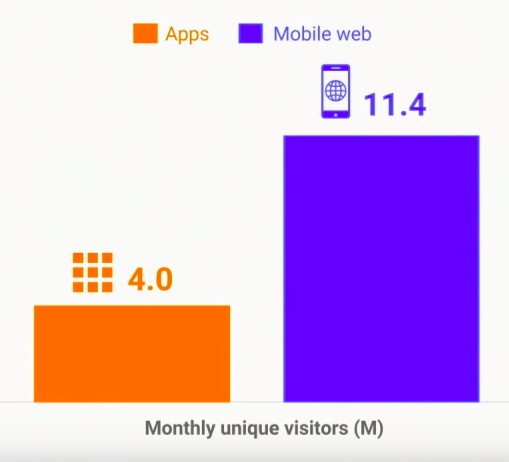
\includegraphics[scale=0.4]{slike/pwa.png}
\end{center}
\caption{Mesečni broj jedinstvenih posetilaca}
\label{fig:pwa}
\end{figure}

Neke prednosti progrsivnih web aplikacija su:
\begin{itemize}
    \item Pouzdanost - odmah se učitavaju i to nezavisno od stanja interneta.
    \item Brzina - brzi odgovori prilikom interakcije sa korisnikom.
    \item Pogodnosti za korišćenje - mogu se instalirati i biti na početnim ekranima korisnika bez potrebe za skidanjem sa Play Store-a ili App Store-a. Ovu funkcionalnost omogućava Web App Manifest.
    \item Raspoloživost - mogu se pokrenuti na mobilnim uređajima, stonim računarima i tabletima.
\end{itemize}

Progresivne web aplikacije su se dobro pokazale i u praksi što dokazuje i to da je nakon ponovnog pokretanja BMW.com kao progrsivna web aplikacija primećeno 3-4 puta brže učitavanje, 30\% više klikova i 26\% više mobilnih korisinka. Isto tako, kada je Trivago predstavio svoju novu progresivnu web aplikaciju, kompanija je zabeležila 50\% povećanje mobilnih sesija zajedno sa 150\% povećanjem aktivnosti korisnika koji su dodali Trivago na početnu stranicu. 

U svom izveštaju za 2017. godinu Gartner je predvideo da će PWA biti najveći trend razvoja softvera u narednim godinama što se obistinilo u 2018. godini.

\subsection{Noviteti u programiranju Android aplikacija}
\label{subsec:noviteti u programiranju Andriod aplikacija}

Što se tiče noviteta u programiranju Android aplikacija treba posebno spomenuti programski jezik Kotlin, koji je 2017. i 2018. godine doživeo veliki uspeh, ali i uveo mnoge novitete koji olakšavaju život programerima, ali takođe pružaju pregršt pogodnih funkcija \cite{kotlin}. Ima dosta sličnosti sa Javom, a jedan od najvećih noviteta koji olakšava programiranje je to da je Kotlin, za razliku od Jave bezbedan što se tiče null vrednosti. Naime, Java omogućava dodeljivanje null vrednosti bilo kojoj promenljivoj, ali prilikom korišćenja reference objekta koji ima null vrednost, onda dolazi do pojave koja najviše frustrira Java programere, a to je NullPointerExceptions. Sa druge strane, u Kotlin-u, svi tipovi su podrazumevano non-nullable tj ne mogu imati null vrednost. Ako pokušamo da dodelimo ili vratimo null u naš Kotlin kod, greška će biti prijavljena za vreme kompajliranja.

Još jedan novitet koji uvodi Kotlin jesu ''coroutine'' \cite{coroutine}. Naime, kada imamo neku dugotrajnu operaciju, nit se blokira dok se ta operacija ne završi, a čim se glavna nit blokira korisnički interfejs će se zamrznuti i aplikacija će ostati neaktivna dok se operacija ne završi. U Javi, rešenje je bilo da se napravi pozadinska nit u kojoj se može izvesti ova dugotrajna operacija, ali upravljanje višestrukim nitima može dovesti do složenog koda koji je sklon greškama, a i kreiranje nove niti je skupa operacija. Ovde na scenu stupaju ''coroutine'' Kotlina koje obavljaju dugotrajne i intezivne zadatke obustavljanjem izvršavanja u određenoj tački bez blokiranja niti, a zatim nastavljanje ove funkcije u sledećoj tački, moguće i na drugoj niti. Ovo nam omogućava da kreiramo asinhroni kod bez blokiranja koji izgleda sinhrono i dosta je jasniji, koncizniji i čitljiviji. ''Coroutine'' su bez steka, tako da upotrebljavaju manje memorije u odnosu na niti i otvaraju vrata dodatnim stilovima asinhronog programiranja bez blokiranja, kao što je async/await.

\subsection{Front end JavaScript okviri}
\label{subsec:front end javascript okviri}

Konačno, bez spominjanja React-a i Angular-a priča o trendovima u programiranju u poslednje vreme je nepotpuna. React i Angular su sve više prihvaćeni od strane dizajnera za dizajn i izradu prototipova korisničkog interfejsa. Oni nude arhitekturu zasnovanu na komponentama i modulima, što dosta utiče na strukturu samih projekata. Njihovom pojavom dizajn sve više postaje baziran na komponentama, a ne orijentisan na ekran. Za Angular je 2018. godina bila od posebnog značaja jer su u 2018. godini izdali novu verziju (Angular 7).

Ono što je veoma interesantno je i to što iako se i React i Angular koriste za praktično istu stvar, popularnost i jednog i drugog okvira su i dalje u konstantnom porastu.

\section{Jupyter Notebook}
\label{sec:jupyter notebok}

Ovu sekciju smo izdvojili da bismo Vas bolje upoznali sa Jupyter Notebook-om. Trenutno se ne nalazi na spisku najtraženijih jezika, nije najviše plaćen, ali je noviji i sa tendencijom da njegova upotreba drastično poraste.

Prvi put smo se sreli sa Jupyter Notebook pre 5 godina tada poznatim kao IPython notebooks, program za organizaciju i analizu podataka. Koristeći Google BigQuery na javnim podacima možemo pronaći koliko puta je Jupyter paket instaliran na PyPi (centralizovan repoiztorijum za Python paketne distribucije) \cite{jupyter}.

\begin{lstlisting}[caption={Broj instalacija Jupyter Python paketa na PyPi},frame=single, label=simple, language=SQL]
SELECT
  STRFTIME_UTC_USEC(timestamp, "%Y-%m") AS yyyymm,
  COUNT(*) as download_count
FROM
  TABLE_DATE_RANGE(
    [the-psf:pypi.downloads],
    DATE_ADD(CURRENT_TIMESTAMP(), -1, "year"),
    CURRENT_TIMESTAMP()
  )
 
WHERE file.project="jupyter"
GROUP BY yyyymm
ORDER BY yyyymm DESC
LIMIT 12
\end{lstlisting}

Rezultat je prikazan u tabeli \ref{tab:tabela1}.

Google BigQuery baza podataka takođe uključuje i podatke sa Stackoverflow-a, pa bi naredni query mogao da nam pokaže potražnju u pitanjima na Stackoverflow-u za Jupyter.

\begin{lstlisting}[caption={Broj pitanja na Stackoverflow-u za Jupyter},frame=single, label=simple, language=SQL]
SELECT tags, COUNT(*) c,  year
FROM (
 SELECT SPLIT(tags, '|') tags, YEAR(creation_date) year
  FROM [bigquery-public-data:stackoverflow.posts_questions] a
  WHERE YEAR(creation_date) >= 2014 AND tags LIKE '%jupyter-notebook%'
)
WHERE tags='jupyter-notebook'
GROUP BY year, tags
ORDER BY year DESC
\end{lstlisting}

Rezultat je prikazan u tabeli \ref{tab:tabela2}.

\begin{table}[h!]
\begin{center}
\caption{Broj instalacija Jupyter Python paketa na PyPi.}
\begin{tabular}{|c|c|c|} \hline
Row& yyyymm& download\_count\\ \hline
1&2018-09&262745\\
2&2018-08&648689\\
3&2018-07&189518\\
4&2018-06&172282\\
5&2018-05&219907\\
6&2018-04&230715\\
7&2018-03&248621\\
8&2018-02&254697\\ \hline
\end{tabular}
\label{tab:tabela1}
\end{center}
\end{table}

\begin{table}[h!]
\begin{center}
\caption{Broj pitanja na Stackoverflow-u.}
\begin{tabular}{|c|c|c|c|} \hline
Row& tags& c& year\\ \hline
1&jupyter-notebook&2247&2018\\
2&jupyter-notebook&2064&2017\\
3&jupyter-notebook&1178&2016\\
4&jupyter-notebook&51&2015\\
5&jupyter-notebook&15&2014\\ \hline
\end{tabular}
\label{tab:tabela2}
\end{center}
\end{table}

Nagli razvoj Jupyter doživljava tek u poslednjih nekoliko godina. Naziv je dobio jer su osnivači pronašli inspiraciju u  Julia (Ju), Pythonu (Py) i R. Za obradu podataka Jupyter je toliko napredovao da je postao standard u toj oblasti, po rečima Lorena Barba, mehanički inženjer na George Washington University.

Jupyter ima dve komponente. Unos korisnika (programerski kod ili tekst) u ćelije na fron-end strani. Pretraživač prosleđuje kod na back-end (kernel) koji pokreće kod i vraća rezultat. Prema osnivaču Perezu, više od 100 Jupyter kernela je napravljeno, koji podržavaju veliku količinu različitih jezika. Notebook može takođe da se pokreće i na cloud-u. Najnovija varijanta Jupytera jeste JupyterLab, čija beta verzija je nastala u januaru 2018. godine i dostupna je ili kao samostalan paket ili kao deo besplatnog Anaconda okruženja.

\section{Zaključak}
\label{sec:zakljucak}

Ovim radom smo pokušali da Vas upoznamo sa najrazvijenijim jezicima sadašnjice kao i da Vam pokažemo okvirne tendencije koji će se jezik razvijati u bliskoj budućnosti. Time možete steći sliku o tome gde je vaš trenutni položaj, da li idete u korak sa industrijom i zahtevima na tržištu. Nismo se bavili konkretnim programskim jezicima koji su doživeli uspeh ponaosob. Na pitanje koji programski jezik treba učiti se ne može dati konkretan odgovor jer to zavisi od zahteva projekta, oblasti kojom se bavite i vaših ličnih preferencija. Iz tih razloga, nemojte se slepo voditi statistikom o razvoju nekog jezika, pažljivo birajte, jer je dobro izabrana tehnologija najbitniji deo svakog projekta.

\addcontentsline{toc}{section}{Literatura}
\appendix
\bibliography{literatura}
\bibliographystyle{unsrt}
\bibliographystyle{plain}

\end{document}
